%!TEX root = ../dokumentation.tex

\chapter{Quiescence Search}\label{ch:quiescence}
Dieses Kapitel beschäftigt sich mit der konkreten Zielsetzung dieser Arbeit: Eine Ergänzung der Schach-KI, sodass die Quiescence Search implementiert ist und das Programm somit effektivere Züge berechnen kann. 

\section{Motivation}\label{section:motivation}
Zunächst gilt zu klären, welche Motivation beziehungsweise welche Problemstellung der Notwendigkeit der Quiescence Search zugrunde liegt. Die Bezeichnung für das Problem, welches bei der vorhandenen Implementierung des Algorithmus auftritt, lautet \textit{Horizonteffekt}. Aufgrund der Tatsache, dass der Algorithmus mit einer festen Tiefe arbeitet, existiert für das Programm ein metaphorischer Horizont, über welchen es nicht hinausschauen kann. \textit{Oxford Reference} definiert den Begriff "`Horizonteffekt"' folgendermaßen: "`\textit{The horizon effect refers to the fact that interesting results will always exist beyond any depth D and therefore in any given search will not be discovered} […]"'\footcite{oxford}.

Abbildung~\ref{fig:problem} zeigt eine beispielhafte Aufstellung der Figuren auf einem Schachbrett. Aufgabe der KI ist es nun, den bestmöglichen Zug zu finden\footnote{Um das Beispiel möglichst einfach zu halten, wird angenommen, dass die KI mit einer Tiefe von $1$ rechnet. Für die Erklärung der Problemstellung macht dies jedoch keinen Unterschied, da sich das Beispiel übertragen lässt}.  Das Programm wird schnell erkennen, dass die Dame auf B2 den Springer auf B7 schlagen kann. Da der Horizont an dieser Stelle "`endet"', schätzt das Programm eben diesen Zug als den besten ein und gibt ihn zurück. Wäre die Suchtiefe jedoch um eine Ebene tiefer gewesen, hätte das Programm diesen Zug ausgeschlossen, da, nachdem die Dame den Springer geschlagen hat, der Läufer auf A8 die Dame direkt schlagen kann. Da eine Dame jedoch deutlich mehr wert ist als ein Springer -- in der vorhandenen Implementierung ist eine Dame 9 Bauern wert, ein Springer jedoch nur 3,2 Bauern -- handelt es sich um einen sehr schlechten Zug.

\begin{figure}[H]
	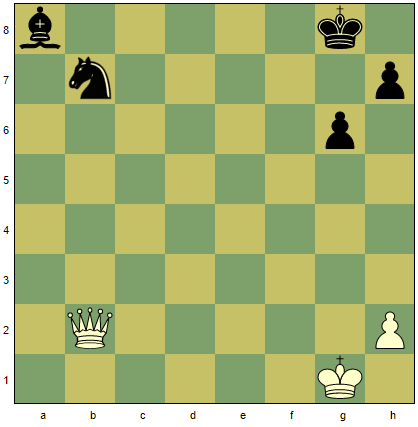
\includegraphics[width=.90\textwidth]{problem.png}
	\caption{Beispiel-Zustand für ein Schachbrett: Weiß kann im nächsten Zug einen Springer schlagen\footnotemark}
	\label{fig:problem}
\end{figure}
\footnotetext{\cite{nextchessmove}}

Ein weiteres Beispiel für den Horizonteffekt ist die scheinbare Vermeidung von schlechten Positionen: Das Programm erkennt eine schlechte Position, beispielsweise den Verlust einer Dame. Nun errechnet die KI einen Pfad, in dem diese Dame scheinbar nicht verloren wird; in der Realität hat das Programm den Verlust jedoch nur "`über"' den Horizont geschoben, sodass der Verlust der Dame unausweichlich ist -- zusätzlich hat das Verschieben des Problems womöglich eine insgesamt schlechtere Position hervorgerufen, als wenn die Dame direkt geopfert worden wäre.

Diese Beispiele verdeutlichen, dass, bei taktischen Zügen, eine tiefere Evaluation nicht nur sinnvoll sondern auch notwendig ist, um die Effektivität der Schach-KI zu steigern. Wird bei der tieferen Evaluation festgestellt, dass der Zug keine schlechtere Position hinter dem Horizont hervorruft, spricht man von einer \textit{ruhigen} Stellung, was auch die Bezeichnung der \textit{Ruhesuche} erklärt.

\section{Funktionsweise}
Bevor die Quiescence konkret implementiert werden kann, muss geklärt werden, wie sie funktioniert und wann sie eingesetzt wird.

In Abschnitt~\ref{section:motivation} wurden \textit{taktische Züge} erwähnt. Das \textit{Chess Programming Wiki} definiert den Begriff folgendermaßen: "`\textit{Tactical moves in the context of chess program move classification are moves which immediate change material balance and capture a piece or cause a promotion} […]"'\footcite{chessprogramming}. Es handelt sich also bei taktischen Züge um das Schlagen von Figuren respektive um das Aufwerten eines Bauern. 

\section{Implementierung}
tbd